%!TEX root = ../main.tex

\section{TensorFlow 简易教程}
\begin{frame}{\secname}
\vfill\hspace{20pt}
\begin{minipage}[m]{0.35\textwidth}
  \linespread{1}\large
  \tableofcontents[sectionstyle = hide/hide, subsectionstyle = show/show/hide]
\end{minipage}%
\hfill%
\begin{minipage}[m]{0.5\textwidth}
  
\includegraphics[height = 7cm]{./icons/lesson.pdf}
\end{minipage}%
\vfill
\end{frame}

\subsection{TensorFlow 简介}
\begin{frame}{\insertsection}{\insertsubsection}
    \tensorflow{} 是一款通过数据流图进行数值计算的开源库. \tensorflow{}  最早是被 Google Brain 的研究者和工程师开发出来的用于机器学习和深度神经网络的研究. 但是这个系统也同样适用于其他领域.

    \tensorflow{} 具有很多非常好的特性:%
    %
    \begin{itemize}
        \item \textbf{易用性}, \tensorflow{} 封装了很多复杂运算, 使用者只需构建计算图.
        \item \textbf{可移植性}, \tensorflow{} 支持多种平台, 系统以及硬件.
        \item \textbf{自动求导}, \tensorflow{} 支持自动求导, 给采用基于梯度下降的学习方法带来了极大便利.
        \item \textbf{支持多种语言}, \tensorflow{} 提供易用的 Python 接口, 也支持 C++, Java, Go 等语言.
        \item \textbf{性能最大化}, 可以部署到不同硬件, 并使用线程, 队列, 异步计算来最大化硬件使用效率.
    \end{itemize}
\end{frame}

\begin{frame}{\insertsection}{\insertsubsection}
    \begin{table}[!htb]
        \centering
        \begin{tabu}{X[l, -1]|X[l]}
            \tabucline[1pt]{-}
            编程模型 & Dataflow-Like Model\\\hline
            语言     & Python, C++, Go, Rust, Haskell, Java, Julia, JavaScript, R\\\hline
            部署     & Code-once, run everywhere\\\hline
            计算资源 & CPU, GPU, TPU\\\hline
            实现方式 & Local Implementation, Distributed Implementation\\\hline
            平台支持 & Google Cloud Platform, Hadoop File System\\\hline
            数学表达 & Math Graph Expression, Auto Differentiation\\\hline
            优化     & Common Subexpression Elimination,\\
                     & Asynchronous Kernel Optimization,\\
                     & Communication Optimization,\\
                     & Model Parallelism, Data Parallelism, Pipeline\\
            \tabucline[1pt]{-}
        \end{tabu}
    \end{table}
\end{frame}

\subsection{张量 Tensor}
\begin{frame}{\insertsection}{\insertsubsection}
张量最初是个物理学的概念:
\begin{quote}
    A tensor is something that transforms like a tensor\\
    一个量, 在不同的参考系下按照某种特定的法则进行变换, 就是张量.\\
    \rule{0pt}{0pt}\hfill  --- A. Zee, "Einstein Gravity in a Nutshell"
\end{quote}

\pause
在 \tensorflow{} 中, 可以将张量理解成多维数组, 张量穿梭在数据流图中, 当经过节点时, 会被节点按照特定法则变换成另一个张量, 这个就是 \tensorflow{} 名字的由来.

\pause
张量的维数被称为张量的阶, 我们常见的标量, 其实是 $0$ 阶张量, 矢量就是 $1$ 阶张量, 矩阵就是 $2$ 阶张量, 一幅图片, 在 \tensorflow{} 中可以是 $3$ 阶张量.
\end{frame}

\begin{frame}{\insertsection}{\insertsubsection}
\tensorflow{} 文档中使用了三种记号来方便地描述张量的维度: 阶, 形状以及维数. 下表展示了他们之间的关系:\vspace{10pt}

\begin{table}
  \centering
  \begin{tabu}{clcl}
  \tabucline[1pt]{-}
  \rowfont{\bfseries}
  阶       & 形状                                     & 维数     & python 代码\\
  \hline
  $0$      & \texttt{[ ]}                             & $0$      & \inlinepython{t0 = 483}\\
  $1$      & \texttt{[$D_0$]}                         & $1$      & \inlinepython{t1 = [1.1, 2.2, 3.3]}\\
  $2$      & \texttt{[$D_0$, $D_1$]}                  & $2$      & \inlinepython{t2 = [[1, 2, 3], [4, 5, 6], [7, 8, 9]]}\\
  $3$      & \texttt{[$D_0$, $D_1$, $D_2$]}           & $3$      & \inlinepython{t3 = [[[1], [2]], [[3], [4]], [[5], [6]]]}\\
  $\vdots$ & $\vdots$                                 & $\vdots$ & $\vdots$\\
  $n$      & \texttt{[$D_0$, $D_1$, $\cdots$, $D_n$]} & $n$      & \inlinepython{tn = ...}\\
  \tabucline[1pt]{-}
  \end{tabu}
\end{table}
\end{frame}

\begin{frame}{\insertsection}{\insertsubsection}
除了维度, Tensors 有一个数据类型属性. 可为一个张量指定下列数据类型的任意一个类型:\vspace{10pt}

\begin{table}
  \centering
  \begin{tabu}{ll|ll}
  \tabucline[1pt]{-}
  \rowfont{\bfseries}
  类型 & 描述 & 类型 & 描述 \\
  \hline
  \inlinepython{tf.float32} & 32 位浮点数     & \inlinepython{tf.string}    & 可变长度的字节数组\\
  \inlinepython{tf.float64} & 64 位浮点数     & \inlinepython{tf.bool}      & 布尔型\\
  \inlinepython{tf.int64}   & 64 位有符号整型 & \inlinepython{tf.complex64} & 由两个 32 位浮点数组成的复数\\
  \inlinepython{tf.int32}   & 32 位有符号整型 & \inlinepython{tf.qint32}    & 用于量化操作的 32 位有符号整型\\
  \inlinepython{tf.int16}   & 16 位有符号整型 & \inlinepython{tf.qint8}     & 用于量化操作的 8 位有符号整型\\
  \inlinepython{tf.int8}    & 8 位有符号整型  & \inlinepython{tf.quint8}    & 用于量化操作的 8 位无符号整型\\
  \inlinepython{tf.uint8}   & 8 位无符号整型  & & \\
  \tabucline[1pt]{-}
  \end{tabu}
\end{table}
\end{frame}

\begin{frame}[fragile]{\insertsection}{\insertsubsection}
\tensorflow{} 中张量包括 \inlinepython{constant}, \inlinepython{placeholder} 和 \inlinepython{Variable}.

\begin{onlyenv}<2>
\inlinepython{tf.constant()} 函数提供在 \tensorflow{} 中定义不可更改张量的方法, 定义如下所示.

\begin{pythoncode}
def constant(value, dtype=None, shape=None, name="Const", verify_shape=False)
\end{pythoncode}

\begin{itemize}
\item \inlinepython{value}, 符合 \tensorflow{} 中定义的数据类型的常数值或者常数列表;
\item \inlinepython{dtype}, 数据类型, 可选;
\item \inlinepython{shape}, 常量的形状, 可选;
\item \inlinepython{name}, 常量的名字, 可选;
\item \inlinepython{verify_shape}, 常量的形状是否可以被更改, 默认不可更改.
\end{itemize}

除了直接赋值以外, 还可使用 \inlinepython{tf.ones()}, \inlinepython{tf.zeros()} 等初始化张量的方法.
\end{onlyenv}

\begin{onlyenv}<3>
\inlinepython{tf.placeholder()} 函数提供在 \tensorflow{} 中定义占位张量的方法, 定义如下所示.

\begin{pythoncode}
def placeholder(dtype, shape=None, name=None)
\end{pythoncode}

\begin{itemize}
\item \inlinepython{dtype} 指定占位张量的数据类型, 可以是 \tensorflow{} 中的数据类型, 如常用的 \inlinepython{tf.float32}, \inlinepython{tf.float64} 等数值类型;
\item \inlinepython{shape} 表示数据类型, \inlinepython{shape = [None, 5]}, 表示行不定, 列是 \inlinepython{5};
\item \inlinepython{name} 是张量名称;
\end{itemize}

占位变量是一种 \tensorflow{} 用来解决读取大量训练数据问题的机制, 它允许你现在不用给它赋值, 随着训练的开始, 再把训练数据传送给训练网络学习.
\end{onlyenv}

\begin{onlyenv}<4->
\tensorflow{} 中变量是通过 \inlinepython{Variable} 类来实现的, 初始化函数定义如下.

\begin{pythoncode}
def __init__(self, initial_value=None, trainable=True, collections=None, validate_shape=True, caching_device=None, name=None, variable_def=None, dtype=None, expected_shape=None, import_scope=None)
\end{pythoncode}


\only<4>{
\begin{itemize}
\item \inlinepython{initial_value}, 初始值, 必填, 张量或可以转换为张量的 Python 对象;
\item \inlinepython{trainable}, 如果参数 \inlinepython{trainable} 的值为 \inlinepython{True}, 则默认值也将变量添加到图形中集合 \inlinepython{GraphKeys.TRAINABLE_VARIABLES}. 这个集合用作 \inlinepython{Optimizer} 类使用的默认变量列表;
\item \inlinepython{collections}, 新的变量被添加到这些集合. 默认为 \inlinepython{[GraphKeys.GLOBAL_VARIABLES]};
\end{itemize}
}
\only<5>{
\begin{itemize}
\item \inlinepython{validate_shape}, 如果 \inlinepython{False}, 允许变量用初始化未知形状的值. 如果 \inlinepython{True}, 默认的形状 \inlinepython{initial_value} 必须是已知的;
\item \inlinepython{caching_device}, 指定变量的默认缓存位置;
\item \inlinepython{name}, 是张量名称;
\end{itemize}
}
\only<6>{
\begin{itemize}
\item \inlinepython{variable_def}, 指定 \inlinepython{VariableDef} 的协议缓冲区;
\item \inlinepython{dtype}, 指定张量的数据类型;
\item \inlinepython{expected_shape}, 是张量的形状, 如果设置, \inlinepython{initial_value} 需要符合这个形状;
\item \inlinepython{import_scope}, 张量名称前缀.
\end{itemize}
}

\end{onlyenv}
\end{frame}

\subsection{节点 Operator}
\begin{frame}{\insertsection}{\insertsubsection}
在 \tensorflow{} 中, 每一个节点代表着一个操作, 一般用来表示施加的的数学运算, 也可以表示数据输入的起点以及输出的终点. 下面是一些重要的操作:\vspace{-15pt}

\begin{table}
  \centering
  \begin{tabu}{ll|ll}
  \tabucline[1pt]{-}
  \rowfont{\bfseries}
   操作 & 描述 &  操作 & 描述 \\
  \hline
  \inlinepython{tf.add(x, y, name=None)} & 求和 & \inlinepython{tf.sign(x, name=None)}   & 返回符号\\
  \inlinepython{tf.sub(x, y, name=None)} & 减法 & \inlinepython{tf.neg(x, name=None)}    & 取负 ($y = -x$)\\
  \inlinepython{tf.mul(x, y, name=None)} & 乘法 & \inlinepython{tf.square(x, name=None)} & 计算平方 ($y = x^2$)\\
  \inlinepython{tf.div(x, y, name=None)} & 除法 & \inlinepython{tf.round(x, name=None)}  & 求最接近的整数\\
  \inlinepython{tf.mod(x, y, name=None)} & 取模 & \inlinepython{tf.sqrt(x, name=None)}   & 开根号 ($y = \sqrt{x}$)\\
  \inlinepython{tf.pow(x, y, name=None)} & 乘幂 & \inlinepython{tf.abs(x, name=None)}    & 绝对值\\
  \inlinepython{tf.inv(x, name=None)}    & 取反 & \inlinepython{tf.exp(x, name=None)}    & 计算 $\e$ 的次方\\
  \tabucline[1pt]{-}
  \end{tabu}
\end{table}
\end{frame}

\subsection{数据流图 Graph}
\begin{frame}{\insertsection}{\insertsubsection}
\vspace{10pt}
\begin{minipage}[m]{0.5\textwidth}
    \tensorflow{} 是用数据流图对计算过程进行描述的. 在数据流图中, 节点代表数学运算, 边表示节点之间的某种联系, 负责在节点之间传输即张量.

    节点可以被分配到多个计算设备上, 可以异步和并行的进行操作. 因为是有向图, 所以只能等待之前的节点运行结束, 当前节点才能执行操作.

    如图所示是一个简单的数据流图.%
    \end{minipage}\hfill
    \begin{minipage}[m]{0.4\textwidth}
    \inlineframe{\scalebox{0.8}{%!TEX root = ../main.tex

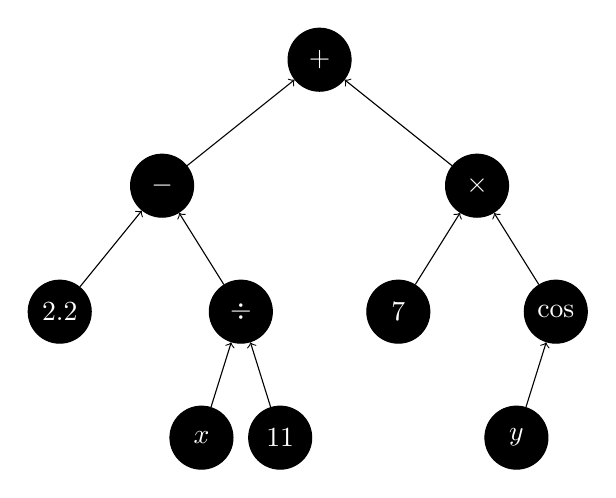
\begin{tikzpicture}[%
    node/.style = {circle, draw, minimum size = 0.8cm, align = flush center, inner sep = 0pt, fill = black, text = white},
    y = 0.8cm]

    \node[node] (x) at (5, 0) {$x$};
    \node[node] (11) at (6, 0) {$11$};
    \node[node] (y) at (9, 0) {$y$};
    \node[node] (div) at (5.5, 2) {$\div$};
    \node[node] (22) at (3.2, 2) {$2.2$};
    \node[node] (7) at (7.5, 2) {$7$};
    \node[node] (cos) at (9.5, 2) {$\cos$};
    \node[node] (sub) at (4.5, 4) {$-$};
    \node[node] (times) at (8.5, 4) {$\times$};
    \node[node] (plus) at (6.5, 6) {$+$};

    \draw[->] (x) -- (div);
    \draw[->] (11) -- (div);
    \draw[->] (y) -- (cos);
    \draw[->] (22) -- (sub);
    \draw[->] (div) -- (sub);
    \draw[->] (7) -- (times);
    \draw[->] (cos) -- (times);
    \draw[->] (sub) -- (plus);
    \draw[->] (times) -- (plus);
\end{tikzpicture}
}}
    \[
        \text{表达式: }\bigg(2.2 - \Big(\frac{x}{11}\Big)\bigg) + \big(7 \times \cos(y)\big)\text{.}
    \]
\end{minipage}
\end{frame}

\begin{frame}[fragile]{\insertsection}{\insertsubsection}
\begin{pythoncode}
import tensorflow as tf
import numpy as np

x1 = tf.placeholder(tf.float32, [None, 1])
w1 = tf.Variable(tf.random_normal([1, 10]))
b1 = tf.Variable(tf.ones([1, 10]))

x2 = tf.nn.relu(tf.matmul(x1, w1) + b1)
w2 = tf.Variable(tf.random_normal([10, 1]))
b2 = tf.Variable(tf.ones([1, 1]))

predicted_values = tf.matmul(x2, w2) + b2
actual_values = tf.placeholder(tf.float32, [None, 1])
loss = tf.reduce_mean(tf.reduce_sum(tf.square(actual_values - predict_values), reduction_indices = [1]))
\end{pythoncode}

\vspace{-7.5cm}\hspace{10.5cm}\scalebox{0.53}{\begin{tikzpicture}[%
  tensor/.style = {rectangle, inner sep = 2pt, rounded corners = 0.4cm, draw, align = flush center, minimum height = 0.8cm, minimum width = 0.8cm},
  operator/.style = {tensor, fill = black, draw = none, text = white, inner sep = 2pt},
  line width = 1pt,
  y = 1.1cm
]
\node[tensor, circle]   (x1) at (9, 0) {$x_1$};
\node[tensor, circle]   (w1) at (7, 0) {$W_1$};
\node[operator]         (t1) at (8, 1) {\mintinline{text}{tf.matmul}};
\node[tensor, circle]   (b1) at (6, 1) {$b_1$};
\node[operator]         (p1) at (7, 2) {\mintinline{text}{tf.add}};
\node[operator]         (r1) at (7, 3) {\mintinline{text}{tf.nn.relu}};
\node[tensor, circle]   (w2) at (5, 3) {$W_2$};
\node[operator]         (t2) at (6, 4) {\mintinline{text}{tf.matmul}};
\node[tensor, circle]   (b2) at (4, 4) {$b_2$};
\node[operator]         (p2) at (5, 5) {\mintinline{text}{tf.add}};
\node[tensor]           (pv) at (5, 6) {\mintinline{text}{predicted_values}};
\node[tensor]           (av) at (8, 6) {\mintinline{text}{actual_values}};
\node[operator]         (sb) at (6.5, 7.5) {\mintinline{text}{tf.sub}};
\node[operator]         (sq) at (6.5, 8.5) {\mintinline{text}{tf.square}};
\node[operator]         (rs) at (6.5, 9.5) {\mintinline{text}{tf.reduce_sum}};
\node[operator]         (rm) at (6.5, 10.5) {\mintinline{text}{tf.reduce_mean}};
\node[tensor]           (ls) at (6.5, 11.5) {\mintinline{text}{loss}};

\draw[->] (x1) -- (t1);
\draw[->] (w1) -- (t1);
\draw[->] (b1) -- (p1);
\draw[->] (t1) -- (p1);
\draw[->] (p1) -- (r1);
\draw[->] (w2) -- (t2);
\draw[->] (r1) -- (t2);
\draw[->] (b2) -- (p2);
\draw[->] (t2) -- (p2);
\draw[->] (p2) -- (pv);
\draw[->] (pv) -- (sb);
\draw[->] (av) -- (sb);
\draw[->] (sb) -- (sq);
\draw[->] (sq) -- (rs);
\draw[->] (rs) -- (rm);
\draw[->] (rm) -- (ls);
\end{tikzpicture}}
\end{frame}

\subsection{会话 Session}
\begin{frame}[fragile]{\insertsection}{\insertsubsection}
构造阶段完成后, 才能启动图. 启动图的第一步是创建一个 Session 对象, 如果无任何创建参数, 会话构造器将启动默认图. 会话会管理 \tensorflow{} 程序运行时的所有资源. 当所有计算完成之后需要关闭会话来帮助系统回收资源, 否则就可能出现资源泄露的问题. \vspace{10pt}

\begin{minipage}[t]{0.48\textwidth}
\begin{pythoncode}
import tensorflow as tf

a = tf.constant([1.0, 2.0])
b = tf.constant([2.0, 3.0])
result = a + b

session = tf.Session()
print(session.run(result))
session.close()
\end{pythoncode}
\end{minipage}%
\hfill%
\begin{minipage}[t]{0.48\textwidth}
\begin{pythoncode}
import tensorflow as tf

a = tf.constant([1.0, 2.0])
b = tf.constant([2.0, 3.0])
result = a + b

with tf.Session() as session:
    print(session.run(result))
# session.close()
\end{pythoncode}
\end{minipage}
\end{frame}